\chapter{Gli Strumenti}

Una volta che il dato è stato memorizzato, strutturato in maniera conforme al tipo di operazione cui sarà soggetto e pulito è il momento che venga utilizzato attivamente.\\
Questo avviene tramite analisi e elaborazioni operate con il supporto di molteplici framework di sviluppo, aventi come fine ultimo l'estrazione di ulteriori informazioni e la trasformazione di ciò che si è ottenuto finora. Solo in questo modo potranno emergere ulteriori aspetti e \textit{insights}, che verranno visualizzate secondo i principi della Data Visualization.

\section{Le Tecniche}

\subsection{Batch Processing}
L'elaborazione batch è l'approccio storico in termine di analisi dati. Consiste in un elaborazione discretizzata nel tempo, operata su segmenti di dataset ricavati da quello totale e applicata a intervalli regolari di tempo. Questo approccio introduce, dunque, una latenza nell'analisi dovuta proprio a questa analisi frammentata.\\
Il processo effettivamente è organizzato in tre fasi:
\begin{itemize}
	\item raccolta di dati nell'intervallo di tempo definito
	
	\item separazione del dato in batches e relativa elaborazione

    \item scrittura del risultato ottenuto sulla supporto di memorizzazione di scelta
\end{itemize} 
Questo approccio è particolarmente adatto ad applicazioni che richiedono una schedulazione che si adatti ai carichi di lavoro del sistema, permettendo di essere eseguita in momenti di ridotto impiego delle risorse, e che utilizzano un elevato numero di dati e transazioni.\\
Tuttavia, per costruzione, non permette analisi dati in tempo reale, che sta diventando in tempi recenti una condizione determinante nella scelta dell'approccio da seguire.

\subsection{Graph Processing}
Un particolare tipo di analisi che opera su strutture a grafo, composte da nodi e vertici. Vista l'efficacia nel descrivere relazioni tra entità del sistema, rappresentate proprio dai rami che connettono i vari elementi del grafo, il loro utilizzo è ora più che mai attuale. I grafi sono, infatti, il migliore mezzo per descrivere il comportamento di una rete, quale potrebbe essere un moderno Social Network o le connessioni attraverso Internet.\\
Questo tipo di elaborazione richiede strumenti ed astrazioni differenti rispetto alle tecniche classiche adottate con dati strutturati, dando origine ad un campo di analisi dati a sé stante.

\subsection{Stream Processing}
L'elaborazione in stream si distingue dalla sua controparte batch per la possibilità di operare su dataset estesi in tempo reale, considerandoli come flussi continui di dati. Questo paradigma richiede l'adozione di opportune astrazioni per poter applicare i classici operatori e trasformazioni insieme a tecniche di esecuzione per trattare il dato:
\begin{itemize}
	\item \textbf{Stream}: elaborazione senza soluzione di continuità, coerentemente con i flussi di dati generati.
	\item \textbf{Micro-Batch}: approccio non sempre perseguibile, qualora fossero richiesti certi livelli di latenza e consumi di risorse, effettua una partizione del dato in batch di dimensioni ridotte, adottando una soluzione adattata di quanto visto in precedenza.
\end{itemize}
\pagebreak

\section{Hadoop MapReduce}

MapReduce \cite{hadoop_doc} è un framework componente della suite di prodotti Hadoop. È pensato per l'esecuzione su architetture di tipo cluster per lo sviluppo di applicazioni di elaborazione di dati in batches da supporti di memorizzazione distribuiti, che si tratti di filesystem o database. Il nome deriva dal paradigma classico offerto dalle operazioni \textit{map} e \textit{reduce}, derivate dai dettami della programmazione funzionale.\\\\
Utilizza un'architettura con primitive che lavorano "on disk", ossia che richiedono la presenza del dato su disco. Sebbene questo sia un vantaggio in termini economici e si sposi con l'elaborazione batch che vuole soddisfare, questo approccio introduce importanti tempi di latenza, dovuti proprio alla necessità di continue operazioni di lettura e scrittura su un supporto a lente transizioni quale è il disco.\\ 
Proprio per questo, con la sempre più preponderante richiesta di elaborazioni in tempo reale, MapReduce sta lentamente perdendo l'appeal che aveva originariamente, pur rimanendo la scelta prediletta per il batch processing.

\subsection{Struttura}
Per operare in maniera distribuita necessita di due componenti:
\begin{itemize}
	\item \textbf{Job Tracker}: ricopre il ruolo principale di \textit{master} e funge da centro di controllo dell'elaborazione, reagendo a errori del sistema tramite un'opportuna rischedulazione dei task. Si occupa di gestire le risorse a disposizione, che vengono distribuite a chi ne necessiti. Per ottimizzare i tempi di esecuzione viene data precedenza alle operazioni che richiedono dati già presenti nel filesystem o che siano in un nodo vicino, riducendo quanto possibile i tempi di latenza. 
	
	\item \textbf{Task Trackers}: rappresentano gli \textit{slaves} della struttura e lavorano su ciascun nodo, dove eseguono i compiti assegnati dal Job Tracker.
\end{itemize}

\pagebreak

\section{Apache Spark}
Apache Spark \cite{spark_doc} è un framework open source per il calcolo distribuito in tempo reale, nato a Berkeley nel 2009 e successivamente passato sotto l'ala della Apache Software Foundation, che si occupa tuttora del suo mantenimento.\\ Grazie alle sue caratteristiche ha un ampio spettro di applicazioni, dal Batch Processing al Graph Processing e Stream Processing.

\subsection{Requisiti} 
Il framework richiede un'ambiente che lo supporti nell'interazione con il resto dell'architettura: un gestore di cluster e un sistema di archiviazione distribuita.\\ 
Per quanto riguarda il primo sono supportati Hadoop YARN o Apache Mesos, in aggiunta ai quali è possibile adottare l'opzione \textit{standalone}, consigliata solo con obiettivi di testing, in cui è Spark che avvia i nodi su cui eseguire l'applicazione. In ogni caso il framework è completamente astratto da questo aspetto, unificando l'approccio per ogni scelta adottata.\\
Per il secondo punto il framework richiede uno tra cui i principali rappresentanti della categoria, tra i quali i già citati HDFS o Cassandra.

\subsection{Architettura}
Spark adotta un'architettura distribuita di tipo "Master Slave": un task \textit{Driver} e molteplici tasks \textit{Worker}.\\ 
Il programma \textit{Driver} viene eseguito sul nodo principale e gestisce la divisione delle operazioni sugli altri nodi tramite l'oggetto \textit{SparkContext}. Questo interagisce con il gestore del cluster del sistema per definire job \textit{Executors} nei nodi secondari. A questi vengono successivamente inviati il codice dell'applicazione e i task particolari da eseguire.\\
I programmi \textit{Worker} vengono avviati sui nodi secondari e rimangono in esecuzione per tutta la durata dell'applicazione. È importante sottolineare che ogni applicazione genera processi indipendenti dalle altre, garantendone l'isolazione reciproca per lo scheduling. Tuttavia ciò significa che l'unico modo per far comunicare applicazioni in esecuzione contemporanea consiste nella scrittura su memoria esterna.

\begin{figure}[h]
	\centering
	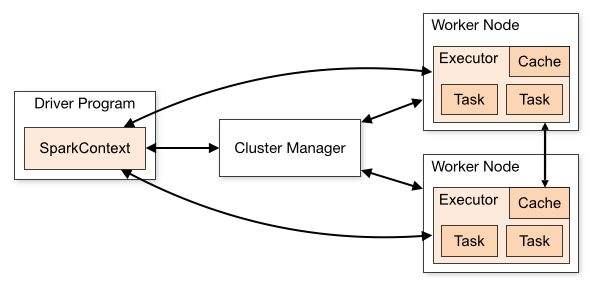
\includegraphics[scale=0.75]{Figures/spark_architecture.png}
	\decoRule
	\caption[Architettura Spark]{Architettura Master Slave}
	\label{fig:Architettura Spark}
\end{figure}

\subsection{Caratteristiche}
Spark si pone nel panorama del Data Processing come principale concorrente ad Hadoop MapReduce. Infatti, contrariamente alla controparte, fornisce l'opzione per lo Stream Processing e punta sull'analisi in tempo reale.\\
Per fare ciò l'architettura utilizza primitive "in-memory", lavorando direttamente in RAM laddove possibile. Questo approccio riduce di molto i tempi di latenza, rimuovendo l'overhead della scrittura su disco. Proprio per queste caratteristiche Spark viene preferito per algoritmi di apprendimento automatico e analisi dati interattiva, che richiedono accesso ripetuto agli stessi dati.

\subsection{Struttura}
Spark è organizzato su due livelli di librerie: uno fondamentale costituito da Spark Core e uno composto dalle estensioni incluse nativamente. Tra le principali in questa situazione riconosciamo:
\begin{itemize}
	\item \textbf{Spark SQL}, per l'interazione con dati strutturati
	\item \textbf{Spark Streaming}, orientata allo Stream Processing
	\item \textbf{MLlib}, che fornisce algoritmi di Machine Learning
	\item \textbf{GraphX}, adottata per il Graph Processing
\end{itemize}  

\begin{figure}[h]
	\centering
	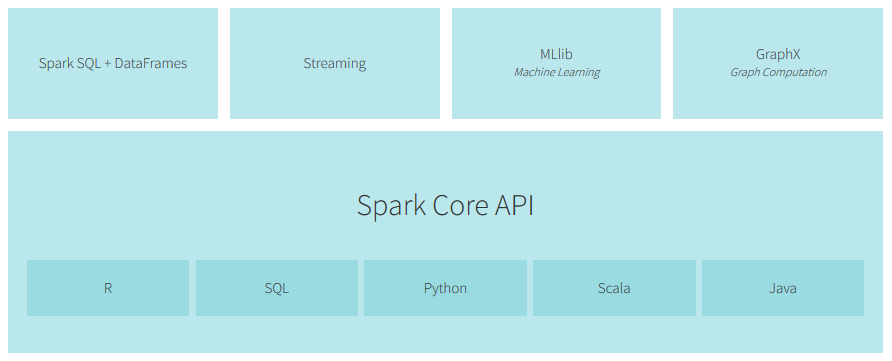
\includegraphics[scale=0.75]{Figures/spark_structure.png}
	\decoRule
	\caption[Struttura Spark]{Struttura Spark}
	\label{fig:Struttura Spark}
\end{figure}

\subsubsection{Spark Core}
Spark Core costituisce le fondamenta dell'intero framework, fornendo metodi di base relativi a scheduling e I/O. Tuttavia tra le componenti principali abbiamo il sopracitato oggetto \textit{SparkContext}, che comunica a Spark come interagire con la struttura del cluster.\\

\begin{code}
	\label{code:SparkContext}
	\begin{minted}[breaklines, breakbefore=., breakafter=(]{Scala}
    val conf = new SparkConf().setAppName(appName).setMaster("yarn")
    val spark = new SparkContext(conf) 
	\end{minted}
\end{code}~\\
È importante ricordare che ogni applicazione può avere solo un oggetto SparkContext attivo alla volta e, pertanto, bisogna ricorrere al metodo \textit{stop()}, qualora ci fosse la necessità di cambiarlo.

\paragraph{RDD} Gli RDDs (Resilient Distributed Datasets) \cite{spark_rdd_doc} sono collezioni di dati immutabili, tipate e distribuite che costituiscono la struttura dati caratteristica di Apache Spark, su cui si basano le ulteriori astrazioni che vengono applicate dalle librerie specifiche (Dataframes, Datasets).\\
Vengono generati a partire da riferimenti ad un sistema di memorizzazione esterno (es. HDFS) o "parallelizzando" una struttura dati già inizializzata nel programma. In questo modo il dato viene suddiviso in base alla struttura distribuita del cluster in partizioni logiche.\\
Supportano due tipi di operazioni: 

\begin{itemize}
	\item \textbf{Trasformazioni}: generano un nuovo RDD che andrà a prendere il posto di quello precedente. Questo perché i RDD sono immutabili in modo da garantire un sistema robusto ai potenziali problemi dovuti all'aggiornamento di risorse parallele. Sono definite "lazy", ossia il risultato non viene calcolato fino a quando non risulta necessario, in modo da evitare inutili sprechi di risorse e ottimizzare l'ordine delle operazioni laddove possibile. Ne sono esempi \textit{map}, \textit{filter} o \textit{join}.
	
	\item \textbf{Azioni} le operazioni che accedono al RDD per restituire un risultato tipato. Sono coloro che innescano l'esecuzione delle trasformazioni. Ne sono esempi \textit{reduce}, \textit{collect} e \textit{count}. 
\end{itemize}
Laddove possibile trasformazioni e azioni vengono effettuate direttamente in memoria, che viene liberata una volta che l'operazione è terminata. Questo garantisce prestazioni decisamente maggiori rispetto ai frameworks che lavorano "on-disk", rimuovendo i pesanti tempi di accesso necessari a interrogare il disco. Tuttavia talvolta può essere richiesto una persistenza del dato in memoria, in modo da rendere le future operazioni su quella risorsa più veloci; questo viene ottenuto tramite i metodi \textit{persist} e \textit{caching}, specificando il livello di memorizzazione necessario (es. MEMORY\_ONLY, DISK\_ONLY). Questa soluzione viene adoperata in particolare per algoritmi iterativi o interrogazioni rapide del dato, in quanto rende le future operazioni sulla risorsa fino a dieci volte più veloci.\\
I RDD godono infine di una politica di "fault tolerance" basata sul concetto di "lineage": viene mantenuta la cronologia delle operazioni  che hanno portato allo stato attuale sottoforma di DAG (Direct Acyclic Graph) e, in caso di errore del sistema, le partizioni vengono ricomputate per ripristinare lo stato corrente. Questo è possibile poiché il meccanismo di partizionamento è un processo deterministico, dunque riproducibile ripercorrendo la storia della risorsa. \newline

\subsection{Estensioni}

\subsubsection{GraphX}

GraphX \cite{spark_graph_doc} è un'estensione di Spark per grafi e analisi su di essi. Utilizza come astrazione di base l'oggetto "Property Graph" derivato dal RDD e mette a disposizione operatori proprietari e operatori ottimizzati derivati dalle API Pregel.

\paragraph{Property Graph}
L'entità Property Graph, o solo Graph, è un multigrafo, cioè un grafo con molteplici rami paralleli con vertici in comune, diretto con proprietà definite per ogni ramo e vertice, semplificando la descrizione di relazioni multiple tra coppie di nodi. GraphX riesce a ottimizzare le risorse per la memorizzazione del grafo relativamente al tipo di dato presente al suo interno, utilizzando tipologie diverse di array specializzati.\\
Derivano dai RDDs, i Property Graph condividono con essi tutte le caratteristiche di base già viste:
 
\begin{itemize}
	\item \textbf{Immutabili}: cambiamenti ai valori di un grafo implicano la creazione di uno nuovo che ne prenderà il posto. Per ottimizzare il processo vengono esclusi dalla ricomputazione tutti quei campi non interessati dalla trasformazione.
	
	\item \textbf{Distribuiti}: sono partizionati tra i processi di esecuzione utilizzando alcune tecniche di partizionamento di vertici.
	
	\item \textbf{Fault-tolerant}: mantengono lo stesso archetipo in materia, utilizzando il concetto di "lineage" per ricreare il grafo nel caso di errori di sistema.
\end{itemize}
Tale legame con il concetto di RDD si riflette nella struttura effettiva del Property Graph, che contiene come attributi due oggetti di tipo VertexRDD e EdgeRDD, versioni ottimizzate per vertici e rami della struttura dati.

\paragraph{Operatori}
In aggiunta all'oggetto Graph, il framework mette a disposizione una serie di operatori di base per applicare trasformazioni e azioni ai grafi. Questi sono riuniti sotto la classe \textit{GraphOps}, ma, se si sta utilizzando la versione in Scala del framework, sono disponibili direttamente come metodi del grafo tramite il meccanismo degli \textit{implicits}. Tra le principali famiglie riconosciamo:

\begin{itemize}
	\item \textbf{Operatori di proprietà}: equivalenti del \textit{map} del RDD, sono versioni specifiche e ottimizzate per operare su rami, vertici o le terne definite da "origine - ramo - destinazione", per considerare ogni istanza di una relazione.
	
	\item \textbf{Operatori strutturali}: operano sulla topologia strutturale del grafo, ad esempio \textit{reverse} o \textit{mask}.
	
	\item \textbf{Operatori di join}: consentono di estendere il grafo con dati provenienti da altri grafi o strutture dati esterne (es. RDD).
\end{itemize}

\subsubsection{Spark SQL}
Spark SQL \cite{spark_sql_doc} è il modulo dedicato all'analisi su dati strutturati e semi-strutturati, combinando le carateristiche di Spark con le ottimizzazioni di SQL in ambito relazionale.

\paragraph{DataFrame} Il DataFrame è l'astrazione che estende il RDD per rappresentare la struttura tabellare, tipica dell'ambiente SQL: è, infatti, fondamentalmente un RDD di righe con uno schema ben definito. Può essere generato da un RDD, deducendone lo schema o utilizzandone uno specificato esplicitamente, o a partire da un file da una sorgente esterna:

\begin{itemize}
	\item Json
	
	\item Csv
	
	\item Parquet
	
	\item JDBC
\end{itemize}

\subparagraph{DataFrame APIs}
I DataFrames implementano APIs sullo stile degli operatori SQL, trasposti nel paradigma introdotto dai RDD. Le \textbf{Trasformations} sono operazioni che danno in ritorno un altro oggetto di tipo DataFrame e sono "lazy", ossia non eseguiti se non quando viene richiesto un risultato tramite una Action. Ne sono alcuni esempi \textit{select()}, \textit{groupBy()} e \textit{join()}. Le \textbf{Actions} sono operazioni che restituiscono oggetti diversi da DataFrame e sono quelle che innescano l'effettiva esecuzione delle Transformations precedenti. Ne sono esempi \textit{count()}, \textit{collect()} e \textit{show()}.

\subparagraph{Ottimizzazione} 
Il connubio tra Spark e SQL permette di sfruttare il meglio di entrambi gli ambienti per generare ottimizzazioni sulle operazioni che riguardano i DataFrames. Queste possono avvenire però solo su dati appartenenti ad una ristretta cerchia:

\begin{itemize}
	\item Tipi di dato numerici
	\item Timestamp e Date
	\item String
	\item Array e Map
	\item Case Class
\end{itemize}
Le ottimizzazioni avvengono tramite due componenti del backend di Spark SQL.\\
\textbf{Catalyst} si occupa dell'ottimizzazione per le query effettuate sui DataFrames. Questo perché la struttura fornisce una gran quantità di metadati rispetto al RDD su cui lavorare. La maggior parte dei miglioramenti vengono effettuati riordinando le operazioni richieste, grazie alla "laziness" delle Trasformations, e effettuando per ogni operazione solo la lettura dei dati necessari.\\
\textbf{Tungsten} offre un servizio di encoding dei dati "off-heap" che, grazie alle limitazioni relative ai tipi di dati utilizzabili, può gestire al meglio quelli permessi. 

\begin{itemize}
	\item Gestisce la serializzazione del dato in memoria, minimizzando lo spazio occupato e velocizzando il processo di serializzazione e deserializzazione.
	\item Riconosce quali operazioni lavorano per righe e quali per colonne, cambiando contesto a seconda della necessità.
	\item Opera "off-heap", in modo da evitare i rallentamenti dovuti alla garbage collection.
\end{itemize}

\paragraph{SQL Literals} Uno dei principali concetti che mette a disposizione Spark SQL è quello dei SQL Literals, che permettono di applicare queries in stile SQL direttamente sui DataFrame, garantendo un legame con le tecnologie precedenti e venendo incontro a chi è abituato al diffuso linguaggio di query. Tutti i principali operatori sono supportati:

\begin{itemize}
	\item SELECT, FROM, WHERE
	\item DISTINCT, HAVING
	\item GROUP BY, ORDER BY
	\item Operatori JOIN
	\item Subqueries
\end{itemize}

\subsubsection{Spark Streaming}
Spark Streaming \cite{spark_stream_doc} è l'estensione che si occupa di elaborazione di dati in tempo reale, sfruttando tutte le potenzialità offerte dall'ambiente Spark. In questo modo le APIs forniscono uno strumento scalabile e "fault-tolerant" per analizzare i dati provenienti da un flusso di dati, garantendo un elevato flusso di produzione. Supporta le principali fonti di "ingestion streams", quali Kafka o NiFi e sorgenti esterne come Amazon Kinesis o filesystems (HDFS, S3).\\
Il dato viene assimilato e organizzato in mini-batches, su cui possono essere effettuate le operazioni tipiche del "Batch Processing", utilizzando funzioni di alto livello quali map, reduce e join. Il risultato può essere poi inoltrato ad un filesystem, un database distribuito o nuovamente come stream di dati.

\begin{figure}[h]
	\centering
	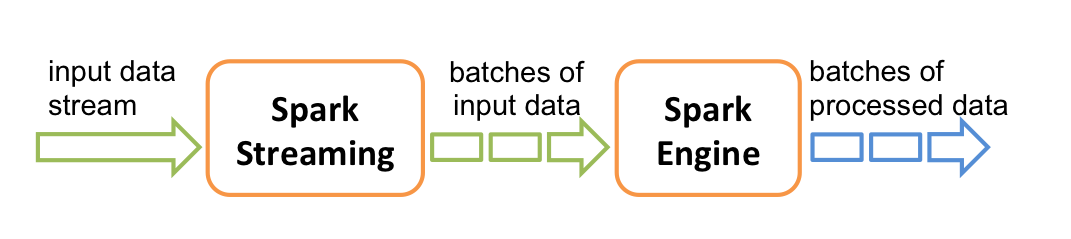
\includegraphics[scale=0.75]{Figures/spark_streaming.png}
	\decoRule
	\caption[Struttura Spark Streaming]{Struttura Spark Streaming}
	\label{fig:Struttura Spark Streaming}
\end{figure}

\paragraph{DStream}
DStream (Discretized Stream) è la principale astrazione utilizzata dalla libreria, che rappresenta uno stream di dati continuo. Può essere generato da una sorgente esterna tra quelle menzionate precedentemente o applicando una trasformazione ad un altro DStream.\\
Le somiglianze con il RDD derivano dal fatto che internamente l'oggetto viene considerato come una sequenza di RDDs, uno per ciascun mini-batch in cui viene discretizzato il flusso di dati in input, mantenendo le caratteristiche di fault-tolerance e parallelismo tipiche della struttura dati che estende.\\
Una volta ottenute le mini-batches, queste passano all'elaborazione con i metodi di Spark, generando corrispondenti batches di dati processati. Questo chiaramente introduce una minima latenza, dovuta alla dimensione del segmento in cui viene suddiviso il flusso di dati.

\subsubsection{MLlib}
La libreria MLLib \cite{spark_mllib_doc} o Machine Learning Library è un estensione di APIs per Spark che fornisce molteplici strumenti e algoritmi per il Machine Learning, con l'obbiettivo di rendere tale approccio semplice e scalabile su grandi moli di dati, sfruttando il paradigma "in-memory" fornito da Apache Spark.\\
Sono disponibili due tipi di APIs, una basata su DataFrame e l'altra su RDD, con quest'ultima che verrà lentamente abbandonata in favore della maggiore semplicità d'uso offerta dal DataFrame.

\paragraph{Gli strumenti} 
MLLib mette a disposizione una pletora di classi e metodi da affiancare agli algoritmi di analisi. Si tratta di classi che spaziano dalla manipolazione e pulizia del dato per adattarlo alla forma richiesta all'ottimizzazione degli iperparametri del modello scelto.

\subparagraph{ML Pipeline} 
Permette di definire le fasi dell'analisi che vogliamo effettuare, raccogliendo i vari passaggi in un'unica sequenza, i \textit{PipelineStages}. In questo modo siamo certi che tutte le operazioni vengano effettuate sul dato, riducendo lo spazio ad errori di sorta.\\
I passaggi possono essere \textit{Transformers}, che trasformano il Dataframe in un altro (es. modificando o aggiungendo colonne), o \textit{Estimators}, astrazione che racchiude tutti gli algoritmi di apprendimento. Mentre gli oggetti \textit{Transformers} implementano solo il metodo \textit{transform()}, usato per applicare l'operazione specificata al dato, gli oggetti di tipo \textit{Estimators} hanno anche un metodo \textit{fit()}, necessario a effettuare il training sui dati specificati e generare il corrispondente modello e diventando un \textit{Transformer}.\\ 
La Pipeline stessa è un \textit{Estimator} e necessita, dunque, di entrambe le operazioni. Una volta definiti gli stages viene chiamato il metodo \textit{fit()}, che viene applicato secondo l'ordine specificato a tutti gli \textit{Estimators} presenti tra gli stages. Viene così generato un \textit{PipelineModel} (o \textit{Fitted Pipeline}), che a questo punto rappresenta una raccolta di soli oggetti \textit{Transformers}. Infine il metodo \textit{transform()} viene applicato su ogni stage sequenzialmente, applicando il modello complessivo al dato considerato.

\subparagraph{ML Tuning} 
Suite di oggetti dedicata all'ottimizzazione dei parametri dei modelli, nota anche come \textit{model selection}. Ne fanno parte:
\begin{itemize}
	\item \textbf{CrossValidator}: classe che applica la tecnica della Cross Validation, congiunta con un ottimizzazione dei parametri specificati del modello. Il dataset viene suddiviso in più partizioni, chiamate \textit{folds}, ognuna delle quali viene alternatamente considerata come testing set e le rimanenti come training set.
	\item \textbf{TrainValidationSplit}: contrariamente alla precedente si concentra solo sull'ottimizzazione dei parametri, effettuando solo una volta la divisione del dataset secondo la frazione specificata.
\end{itemize}
Ciascuno di questi strumenti necessita di tre elementi: 
\begin{itemize}
	\item \textbf{Estimator}: algoritmo o \textit{Pipeline}, soggetto dell'ottimizzazione.
	\item \textbf{ParamMaps}: parametri e relativi intervalli di valori tra cui vogliamo scegliere il modello migliore.
	\item \textbf{Evaluator}: oggetto che fornisce il criterio discriminante nella valutazione. 
\end{itemize}
Il procedimento dunque prevede la suddivisione del dataset secondo la logica specifica. Per ciascuna coppia di training set e testing set ottenuta in questo modo si itera tra i valori specificati dalle \textit{ParamMaps} e viene selezionato il modello migliore, che viene mantenuto come attributo \textit{bestModel} della classe.

\subparagraph{Feature Transformers} 
Oltre a strumenti più prettamente legati all'aspetto pratico dell'analisi del dato, MLlib mette a disposizione oggetti che si occupano di supportare lo sviluppatore nel modificare la forma delle strutture dati in suo possesso in modo da renderle conformi all'algoritmo o modello selezionato.
\begin{itemize}
	\item \textbf{Tokenizer}: suddivide un testo unico nelle singole parole di cui è composto. Nel caso si volesse avere maggiore controllo sul processo di segmentazione si può ricorrere a \textit{RegexTokenizer}, che permette di specificare la regola da utilizzare tramite espressione regolare (regex).
	\item \textbf{Indexers}: permettono di convertire dati non numerici in numerici, per inserirli come input in modelli o altri operatori. A seconda del tipo di dato che ci troviamo a trattare si ricorre a \textit{StringIndexer}, per input testuali, o a \textit{VectorIndexer}, nel caso di un Vector. In entrambi i casi il dato risultato è una codifica univoca in Double, basata sulla frequenza della singola istanza.
	\item \textbf{Bucketizer}: applicato su una colonna a valori continui, genera segmenti di dominio secondo la logica specificata e applica a ogni elemento il valore della partizione corrispondente, discretizzando la misura.
	\item \textbf{VectorAssembler}: genera un'unica colonna di tipo Vector a partire da molteplici colonne. Viene utilizzato per preparare l'input ad alcuni modelli che richiedono una colonna per rappresentare le feature su cui eseguire l'algoritmo.
\end{itemize}

\paragraph{Gli algoritmi}
Una delle caratteristiche più apprezzate di MLlib risiede nella grande quantità di algoritmi di Machine Learning implementati nativamente:
\begin{itemize}
	\item \textbf{Classificazione}: Linear SVM, Naive Bayes
	\item \textbf{Regressione}: Regressione Lineare, GLM
	\item \textbf{Clustering}: K-Means
	\item \textbf{Tree} e \textbf{Ensembles}: Decision Tree, Random Forest, GBT
\end{itemize}
\pagebreak

